% !TeX spellcheck = en_GB

\documentclass[a4paper,12pt,openright,twoside]{report}
\usepackage[italian]{babel}
\usepackage[T1]{fontenc}
\usepackage{indentfirst}
\usepackage{fancyhdr}
%\usepackage{showkeys}
\usepackage{amssymb}
\usepackage{amsmath}
\usepackage{latexsym}
\usepackage{amsthm}
\usepackage{eucal}
%\usepackage{eufrak}
\usepackage{alltt, fancyvrb, url}
\usepackage{amssymb}
\usepackage{cleveref}
\usepackage{graphicx}
\usepackage{subfigure}
\usepackage{wrapfig}
\usepackage{float}


\usepackage{amsmath,amssymb,stmaryrd,mathtools,alltt}
\usepackage{algorithmic, algorithm}
\usepackage[utf8]{inputenc}
\usepackage{fontenc}
\usepackage{url}
\usepackage[a4paper=true]{hyperref}
\usepackage{cleveref,amsmath,amssymb,stmaryrd,mathtools,alltt,algorithm}
\usepackage{amssymb}
\usepackage[italian]{babel}
\linespread{1.3}

\title{Tirocinio curriculare \\svolto presso il\\ DISI - PSLab}
 
\author{Lorenzo Valentini}
%\date{\today}
\date{05/28/2017}

\begin{document}
	
\maketitle

\begin{abstract}
		Il tema da me scelto per il tirocinio corrisponde alla proposta B punto 2.\\\\
	A) Revisione dell'interfaccia grafica 2D/Swing di Alchemist con focus
	sull'usabilità. Questo integra una serie di passi semi-indipendenti,
	di cui più se ne fanno meglio è:\\
	1- stabilizzazione e rilascio del plugin IntelliJ-Alchemist (uscita
	dallo stadio prototipale con una tesi in completamento)\\
	2- sistema per la modifica dello stato dei nodi (attualmente molto
	caotico, è praticamente una proof of concept)\\
	3- revisione del sistema di creazione e modifica degli effetti\\
	
	B) Sperimentazione (studio, installazione e prove) dei seguenti sistemi
	cloud-oriented (uno su tre, ma anche di più):\\
	1- Confronto fra Paas Open Source (e.g. Cloud Foundry, AppScale,
	Tsuru, Apache Stratos …): sviluppo di un’applicazione minimale e deploy
	su due o più PaaS per confrontarne features, pro e contro di ognuno.\\
	2- Docker e Container Scheduling: sviluppo di un’applicazione
	distribuita minimale che sfrutti la containerizzazione e Docker, deploy
	utilizzando due o più framework di scheduling (e.g Docker Swarm,
	Kubernetes, Apache Mesos …) per effettuarne un confronto.\\
	3- Real-Time Data Processing: installazione e prove di strumenti per
	il processing di dati near real-time , e.g Apache Storm, Kafka, Spark …,\\\\
	
	Lo scopo di questo tirocinio è stato incentrato principalmente sull'apprendimento di alcune tecnologie open-sourse  sull'argomento della virtualizzazione di servizi e sistemi utilizzando strumenti per utomatizzare il deploy di questi su varie arcittetture di natura disomogenea riducendo così in questo modo alcune limitazioni e problemi dettati da fattori riguardanti la compatibilità analizzando anche aspetti di ergonomia in campo applicativo.
	Gli esperimenti condotti con questi strumenti sono stati effettuati in vitro su di un singolo calcolatore dove ogni elemento di un architettura distribuita veniva virtualizato su quest'ultimo.

	Obittivo principale nella fase iniziale è stata quella di acquisire familiarità con gli stumenti e le tecnologie del caso di studio, in modo da individuare tramite una fase di analisi sucessiva pregi e i difetti, dopo di che è stato possibile mediante esercitazioni pratiche reperite direttamente dalla documentazione delle varie teocnologie o prodotti ad-hoc per i test, in modo da valutarne sucessivamente alcuni paramerti. In termini generali si è cercato di valutarne alcune caratteristiche: patricità di utilizzo, difficoltà di installazione e limitazioni o potenzialità che li contraddistinguono uno dall'altro ad esempio caratteristiche riguardanti proprio le loro capacità in alcuni ipotetici casi di studio. Per effettuare i vari test sono stati sviluppati alcuni esempi e script di automazione per alcune operazioni in modo da velocizzare alcuni processi e da testare il reale utilizzo di questi strumenti.
	
	
	\chapter*{Indouzione}
	Vi fornirò una breve introduzione su che cosa verrà trattato sucessivamente più in dettaglio all'interno di questo report, in modo da darvi subito, un idea chiara su alcuni concetti che verrano trattati nel  corso della documentazione.\\
	Iniziamo con il descrivere brevemente qual'è il  paradigma architetturale che sta alla base del concetto dei conteiner e quali siano le differenze tra questi e una comune macchina virtuale; poi andremo  più nello specifico applicando ciò visto fino ad ora per capire  come Docker(-whale) applica al suo interno questo pattern architetturale.\\
	Sucessivamente, dopo aver difatto familiarizzato con  Docker sperimentando in prima persona alcune delle sue funzionalità di base anche tramite l'ausilio di esempi, sarà inoltre possibile estendere il concetto di una singola istanza ad un insieme di istanze, dando così vita al concetto di sciame e di sistema didtribuito  
	\href{https://it.wikipedia.org/wiki/Cloud_computing}{iaas(infrastructur as a service)}. 
	Questo non è altro che più istanze di servizi incapsulati in container distribuiti su un cluster di macchine che cooperano grazie al paradigma (master-slave) mettendo in esecuzione una o più istanze di servizi al prorpio interno secondo delle politiche di scheduling per la gestione del carico di lavoro in parte definite dall'utente in parte dipendenti dall'architettura. Non preoccupiamoci se arrivati a questo punto qualche termine ci risulta strano presto cercheremo di fare chiarezza sull'argomento in modo da ottenere risposte hai nostri dubbi.;)
	
	 
\end{abstract}

% mi crea l'indice in modo automatico
\tableofcontents
 
\chapter{Container}
La contiua espansione dei sistemi cloud e la neccessità di poter scalare servizi e applicazioni in modi sempre più efficiente ed in tempi più ridotti, ha fatto si che venisse rivisto il concetto di macchine virtuali che venivano usate per svolgere questo lavoro.\\
Perché virtualizzare un’intera macchina, quando sarebbe possibile isolarne solamente una piccola parte di essa?\\
Questa idea ha condotto gli sviluppatori a trovare delle strade alternative alla virtualizzazione completa e lo stesso Google, confrontandosi con questo problema, ha sviluppato un’aggiunta al kernel Linux chiamata \href{https://en.wikipedia.org/wiki/Cgroups}{\textbf{cgroups}} chiamato “gruppi di controllo” (control groups, cgroups) che permette di gestire l’accesso alle risorse. I control groups permettono di impostare le quote, impostare le priorità e misurare diversi tipi di risorse, quali: la memoria, l’utilizzo della CPU, gli accessi al disco e così via. Questo modulo ha permesso al team di sviluppo californiano di rilasciare software in maniera più veloce, ed economica e con una scalabilità senza precedenti, permettendogli così di creare un contesto di esecuzione isolato, con un alto livello di astrazione, tanto da imporsi come una sorta di sistema operativo semplificato e virtualizzato sul quale sono basate tutte le applicazioni da loro sviluppate.\\
\begin{figure}[H]
	\begin{center}
		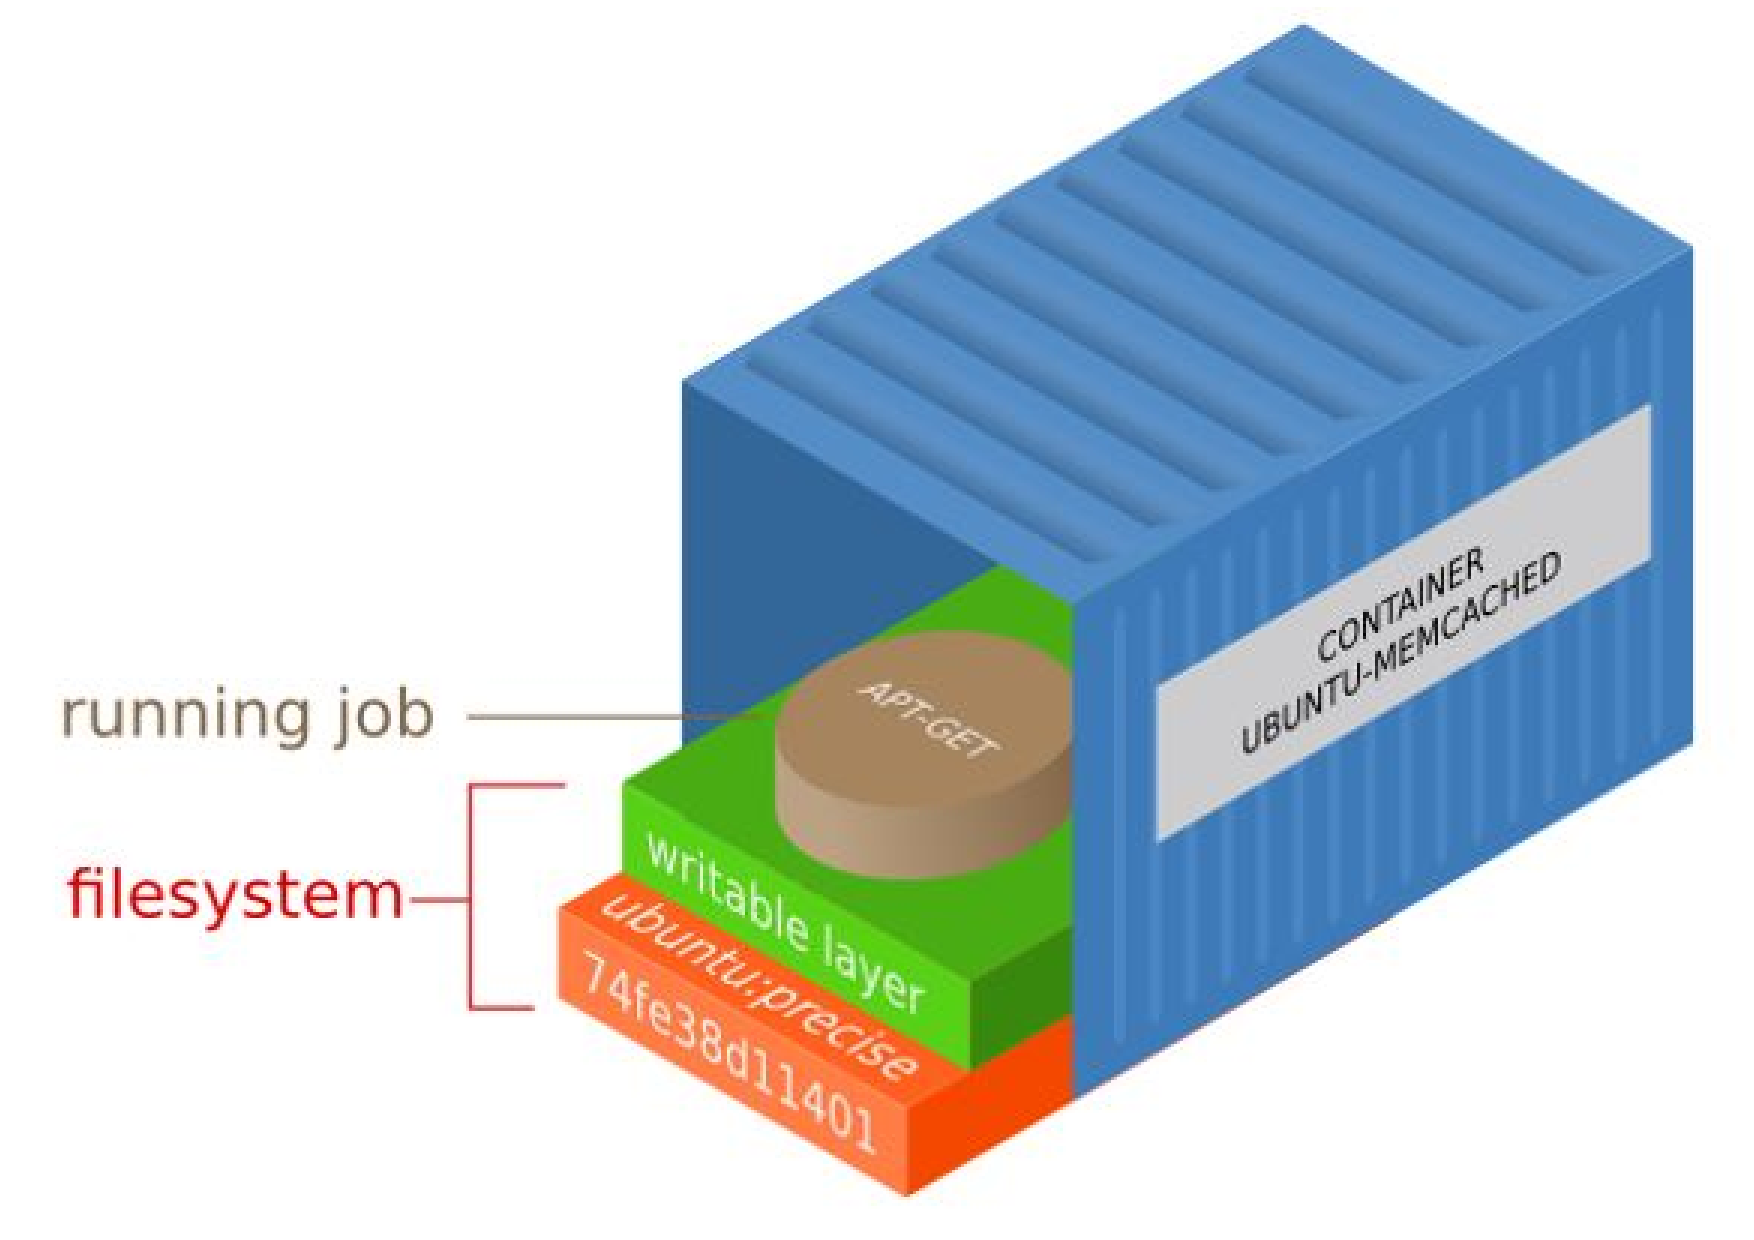
\includegraphics[width=0.99\columnwidth]{img/c.pdf}
		\caption{Interpretazione grafica di un container partendo da un layer di base che comprende un immagine di filesystem ubuntu e uno strato che mostra il livello con i layer personalizzati ed infine l'applicativo o il serviziozio che si vuole utilizzare in esecuzione nel container.}
		\label{img:container}
	\end{center}
\end{figure}
Storicamente, i container sono stati sviluppati nell’ambito del progetto \href{https://linuxcontainers.org/it/lxc/introduction/}{Linux Containers \textbf{LXC}}. Per quanto rappresenti una soluzione valida, \textbf{LXC} non è mai diventata popolare, principalmente per ragioni di usabilità e per la limitata portabilità dei container creati tramite questa tecnologia anche se in alcuni casi specifici preferibili.\\
Dopo pochi anni dai primi sviluppi di questo nuovo paradigma architetturale, la volontà di rendere questa tecnologia uno standard, ha condotto il team di Docker a sviluppare un formato di contenierizzazione interoperabile, capace di pacchettizzare le applicazioni ed effettuarne il deploy in qualsiasi ambiente di esecuzione, senza doversi preoccupare delle condizioni di eseguibilità vedi figura \ref{img:container}.\\
Sucessivamente userò in modo del tutto analogo i termini host e server in caso contrario andrò a difefferenziare i concetti nel dettaglio.
In pratica, la containerizzazione permette di eseguire un qualsiasi \textbf{processo linux} in \textbf{ambiente isolato}.\\
Quindi avremo che un qualsiasi processo "containerizzato" in esecuzione, avrà un proprio \href{https://it.wikipedia.org/wiki/File_system}{\textbf{\emph{ file system}}} privato completamente indipendente da qualsiasi altro processo linux in esecuzione sullo stesso server.
Questo tipo di isolamento potrebbe risultare una limitazione ma in realtà è proprio grazie a questa caratteristica che si riesce a sfruttare una peculiarità del kernel linux ovvero il\href{https://en.wikipedia.org/wiki/Linux_namespaces}{\textbf{namespaces}}, per le quali è possibile  le seguenti risorse:\\
\begin{itemize}
\item\href{https://it.wikipedia.org/wiki/Comunicazione_tra_processi}{\textbf{Inter Process Communications} (IPC)}
\item configurazione di rete
\item il punto di mount della root
\item l’albero dei processi
\item gli utenti e i gruppi di essi
\item la risoluzione del nome di rete
\end{itemize}
Senza addentrarsi in eccessivi tecnicismi, il vantaggio principale sta nel fatto che, con l’uso dei namespace, diventa possibile isolare i processi in modo molto efficace.L’unica cosa che il processo isolato nel container condivide con il sistema operativo ospitante è il kernel Linux.\\\\\\\\\\\\

\section{Paradigma architetturale}
Le differenze sostanziali fra i container e le macchine virtuali sono diverse, entrambe le architeture hanno dei propri pregi e difetti, imputabili all'utilizzo e alle esegenze che essi debbono soddisfare. La creazione di una macchina virtuale è molto diversa da quella di un container poichè lavorano su livelli di astrazione differenti.\\Le VM virtualizzano completamente tutto il sistema dallo strato hardware fino al livello applicativo in modo da andare a ricostruire nel proprio ambiente una vera e propria macchina indipendente dal host su cui essa è ospitata, questa è un'operazione onerosa in termini di tempo e risorse, poichè non banale. Questo fa si che ogni macchina dovrà avere un proprio porzione di memoria centrale, risorse computazionali e un quantitativo di memmoria di massa tutto riservato per e proprie esigenze. Importante portare attenzione al fatto che tutto ciò se per qualche motivo non viene utilizzato rimane allocato per tutto il tempo in cui il sistema virtualizzato rimane in esecuzione privando in questo modo le altre eventuali macchine o applicazioni e servizi in esecuzione sul medesimo server o cluster.\\
Grazie alla tecnologia dei container che non necessita di dover inglobare tutte le risorse di un server, in particolare il kernel del sistema operativo, i container sono molto più “leggeri” delle macchine virtuali, richiedono poche risorse di CPU e possono essere attivati in pochi istanti. Questo li rende particolarmente adatti alle situazioni in cui il carico di elaborazione da sostenere è fortemente variabile nel tempo con picchi di lavoro.
Alcuni scenari appalicativi sono la gestione del traffico per siti web di e-commerce o social-media ma anche in molti altri casi dove numeri elevati di utenti accedono simulotanea e si connettono richiedendo l'utilizzo di alcune risorse o servizi, facendo si che i sistemi siano sottoposti a picchi di connessioni in entrata, che se gestiti in mal modo in certe situazioni potrebbero compromettere la stabilità del sistema e cerete volte rappresentare il fallimento di un progetto o semplicemente il malcontento delle utenze. In questi casi grazie alla tecnologia dei container si possono gestire una moltitudine di richieste attivando in qualche frazioni di secondo un numero elevato di macchine anche decine o centinaia di istanze, ciascuna delle quali esegue il proprio compito gestendo una porzione del carico di lavoro. Un esempio lampante lo si ha nel caso di un web server sul quale esegue un web services, ad un certo punto viene contattato da un numero elevato di visitatori in un breve periodo. esempio "offerte last-minute su un e-commerce" .\\
\begin{figure}[H]
	\begin{center}
		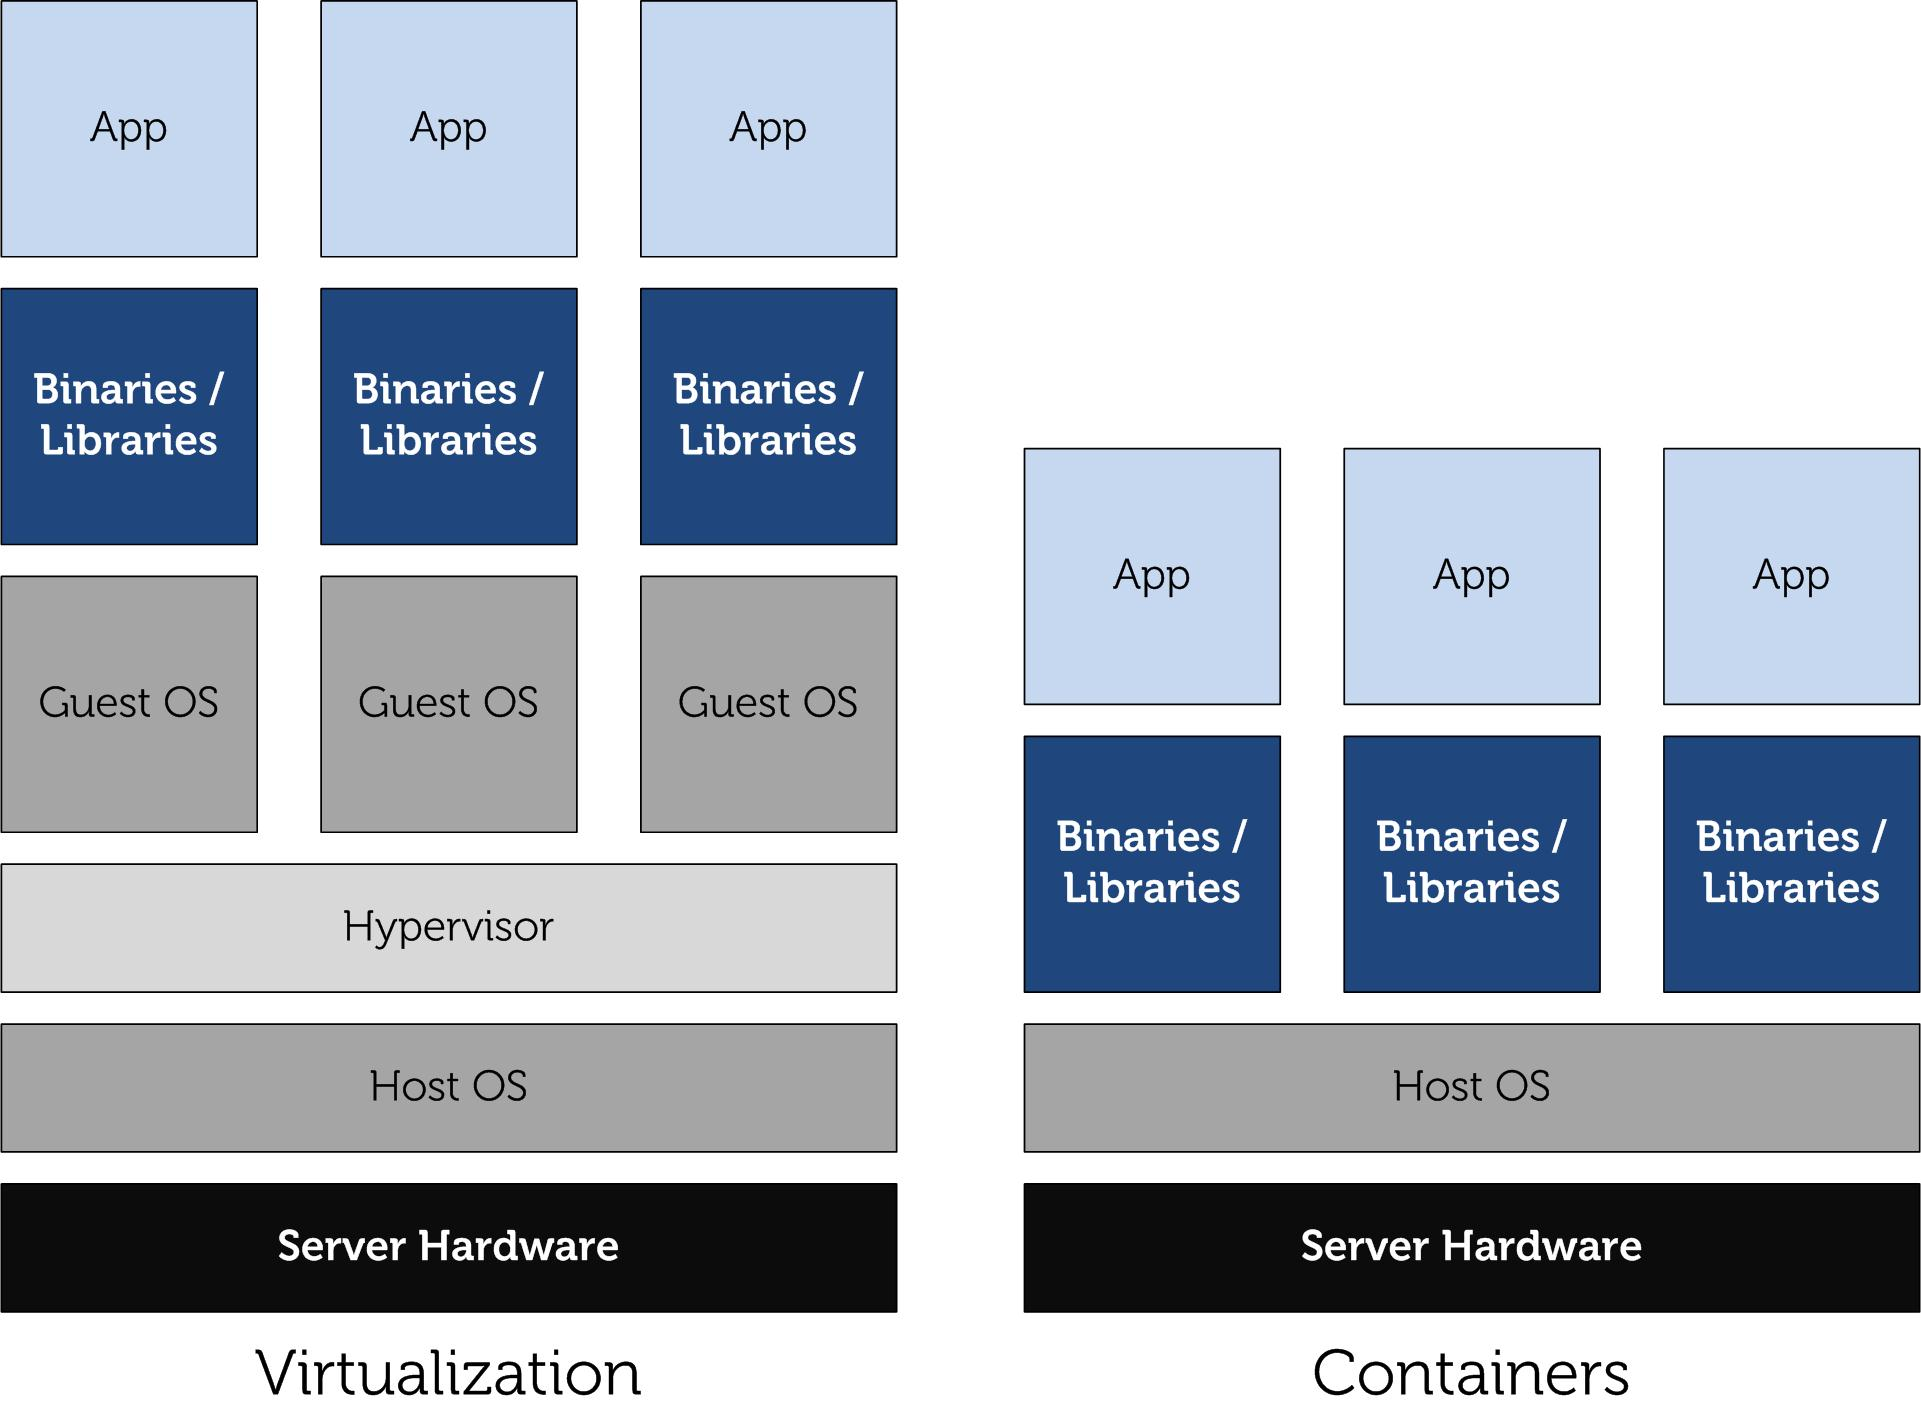
\includegraphics[width=0.99\columnwidth]{img/vm-container.jpg}
		\caption{Container e VM a confronto con le rispettive architetture.}
		\label{img:architettura}
	\end{center}
\end{figure}
Detti alcuni vantaggi offerti da questa nuova tecnologia per ora non ancora attiva sul mercato ma principalmente usata in fase sperimentale ma che nel breve periodo si prevede sostituirà le VM in molti scenari applicativi grazie a queste sue caratteristiche.\\\\\\
I vantaggi della contenierizzazione sono:\\
Poter contenere un numero elevato di container in esecuzione su una singola macchina.\\
Deployment semplificato: impacchettando un’applicazione in un singolo componente distribuibile e configurabile con una sola linea di comando, la tecnologia a container permette di semplificare il deployment di qualsiasi applicazione, senza doversi preoccupare della configurazione dell’ambiente di runtime;\\Una disponibilità rapida: virtualizzando ed astraendo solo il sistema operativo e le componenti necessarie all’esecuzione dell’applicazione, invece che l’intera macchina, l’intero package si avvia in un tempo molto ridotto, rispetto ai tempi di avvio di una VM;\\
Un controllo più granulare: i container consentono agli operatori e agli sviluppatori di suddividere ulteriormente le risorse computazionali in microservizi, garantendo così un controllo superiore sull’eseguibilità delle applicazioni e un miglioramento delle prestazioni dell’intero sistema. Per quanto sia possibile eseguire anche su un laptop diverse virtual machine, questa operazione non è mai veloce e semplice ed impatta sulle sulle prestazioni.\\
Inoltre traggono vantaggi anche sull’amministrazione dei cicli di rilascio delle applicazioni è semplificato, in quanto distribuire una nuova versione di un container è pari al tempo speso per digitare in console una singola linea di comando.\\
Le attività di testing traggono un beneficio economico da un ambiente contenierizzato. Se si effettua il test di un’app direttamente su un cloud server in un ambiente di cloud computing pubblico, sarà necessario sostenere i costi relativi ai tempi di occupazione delle risorse computazionali. Questo costo aumenta all’aumentare del numero di test che devono essere eseguiti. Con un container è possibile effettuare una serie di semplici test programmati mantenendo costante il costo, in quanto si userebbero sempre le stesse risorse di calcolo.
Infine, non si possono ignorare i guadagni in termini di componibilità dei sistemi applicativi, specialmente per le applicazioni open source. In pratica, invece di obbligare gli sviluppatori a installare e configurare i più disparati servizi che potrebbero richiedere molto tempo in termini di messa in installazione come per esempio MySQL, memcached, MongoDB, nginx, node.js e via discorrendo, per avere la giusta piattaforma esecutiva per le proprie applicazioni, sarebbe meno rischioso e più veloce avviare ed eseguire con piccoli script quei pochi container che ospitano queste stesse applicazioni.
Sul lungo periodo, il più importante vantaggio che questa tecnologia promette è la portabilità e la consistenza di un formato che consente l’esecuzione applicativa su diversi host. Infatti, con la standardizzazione dei container, i workload possono essere facilmente spostati lì dove vengono eseguiti in modo più economico e veloce, evitando anche i lock-in (blocchi  e rallentamenti) dovuti alle peculiarità delle piattaforme dei singoli provider.\\Breve panoramica per avere un quadro completo sul fatto che esistono anche container in ambiente Windows, si distinguono in due diversi tipi:

Windows Server Container: forniscono uno strato di isolamento tra gli applicativi usando tecnologie basate sui namespace e la separazione dei processi, ma condividono il kernel tra tutti i container in esecuzione sullo stesso host.

Hyper-V Container: eseguono ogni container in una macchina virtuale ottimizzata, in cui viene eseguita una diversa istanza del kernel non condivisa con gli altri container Hyper-V.\\ 
Il tipo di container utilizzato ha implicazioni anche sul costo della licenza Windows Server.
\subsection{Container vs. Virtual Machine}
In questo caso introduciamo per l'esempio facendo riferimento al modelo architetturale si docker.
\begin{figure}[H]
	\begin{center}
		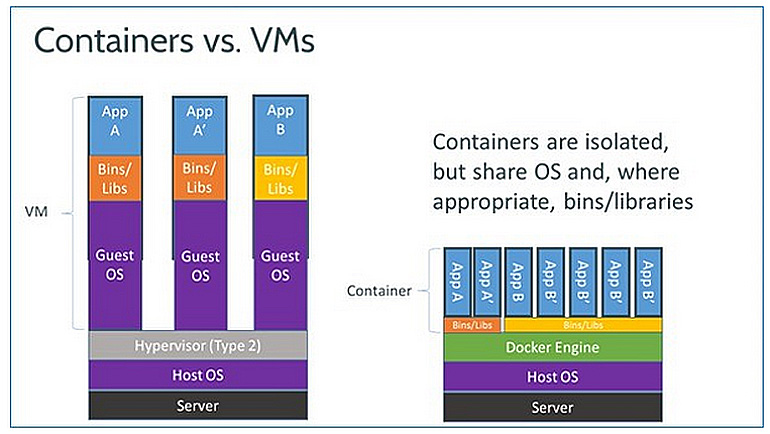
\includegraphics[width=0.99\columnwidth]{img/ContainersOperations-2_fig03.jpg}
		\caption{Container vs. Virtual Machine..}
		\label{img:arch_comp}
	\end{center}
\end{figure}
Come è possibile vedere nella figura \ref{img:arch_comp}, i vantaggi principali dei container si riassumono in un minore consumo di memoria e spazio disco. I container usano meno memoria poiché tutti i container in un ambiente ospitante condividono lo stesso kernel. I container usano meno spazio su disco poiché le immagini dei container possono essere condivise da container che sono in esecuzione sullo stesso host.\\
Dal punto di vista della sicurezza, il consenso generale sembra essere a favore delle macchine virtuali. Infatti le virtual machine appaiono più sicure e più isolate rispetto ai container, ma visto il rapido sviluppo si presume che anche questo cambierà con la progressiva maturazione della tecnologia container.
\section{Docker}
Docker è un progetto open source con una \href{https://www.docker.com/company}{azienda di supporto che fornisce assistenza} e altri servizi a pagamento per la versione docker-EE. La forza di Docker, e una delle ragioni della sua diffusione, è la sua facilità d’uso. Docker è un insieme di tecnologie che cooperano tra loro al fine di standardizzare il formato dei container e avere un insieme di tool standard e funzionanti che permettono di avere la piena portabilità e poter eseguire i container su diverse piattaforme e host.
Le componenti principali di Docker sono:\\
\begin{figure}[H]
	\begin{center}
		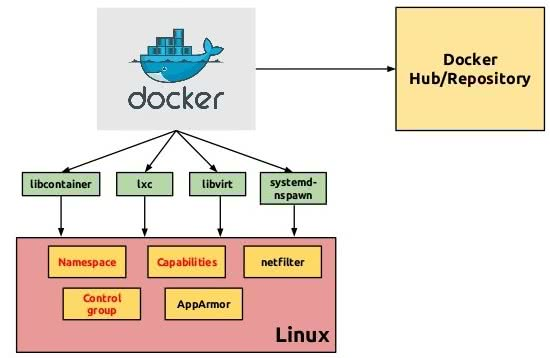
\includegraphics[width=0.99\columnwidth]{img/docker-container_lib.jpg}
		\caption{I registry di Docker.}
		\label{img:API}
	\end{center}
\end{figure}
\begin{itemize}
\item il Docker engine, che è un demone che risiede sul server e accetta comandi da un client (sia da riga di comando sia da chiamate alle API). Esso comunica con il Kernel Linux attraverso la libreria libcontainer (che viene installata insieme a docker).\\
\item il registry, che è una piattaforma che risiede nel cloud e che fornisce un’area dove caricare, scaricare e condividere le immagini dei vari container. Quella ufficiale è \href{https://hub.docker.com/}{https://hub.docker.com}. Supponiamo di voler utilizzare un container con una determinata immagine. Grazie a queste due componenti il cliente chiede al server di prendere quella immagine e “iniettarla” in un container. Il server, se non possiede ancora l’immagine richiesta, contatta il registry. Se esiste nel cloud la scarica e viene creata una copia cache locale. Dopo la inietta in un container. Vedi figura: \ref{img:structDoc1} \ref{img:structDoc2}.\\
\end{itemize}
\begin{figure}[H]
	\begin{center}
		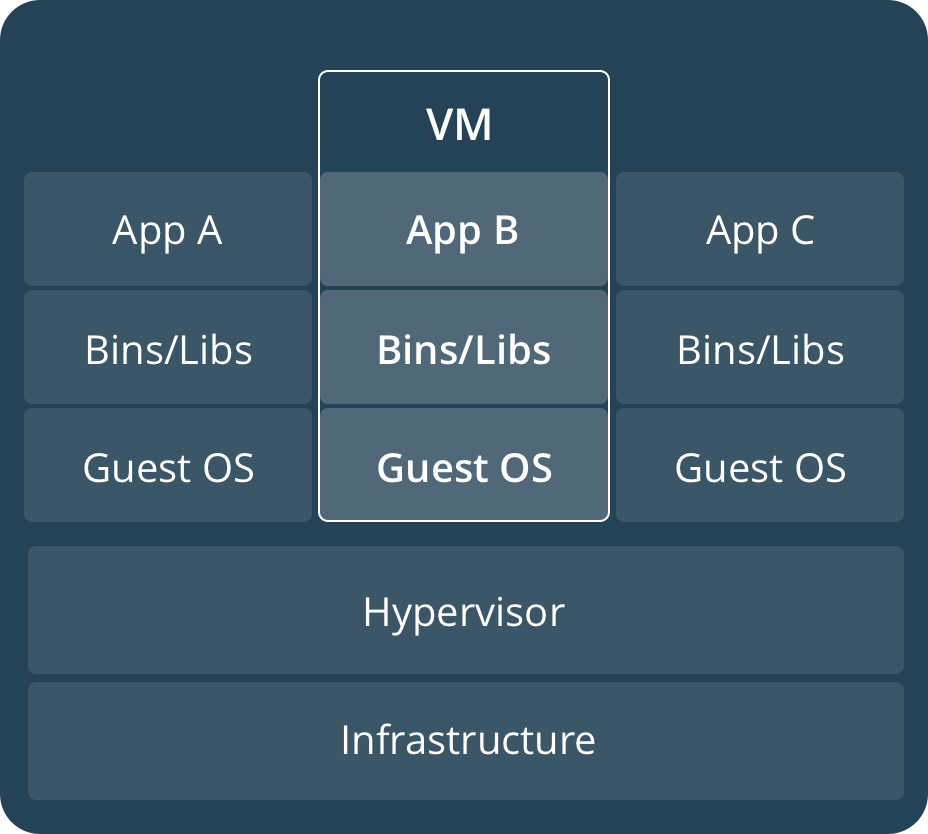
\includegraphics[width=0.70\columnwidth]{img/VM@2x.png}
		\caption{Solution stack classico.}
		\label{img:structDoc1}
	\end{center}
\end{figure}
\begin{figure}[H]
	\begin{center}
		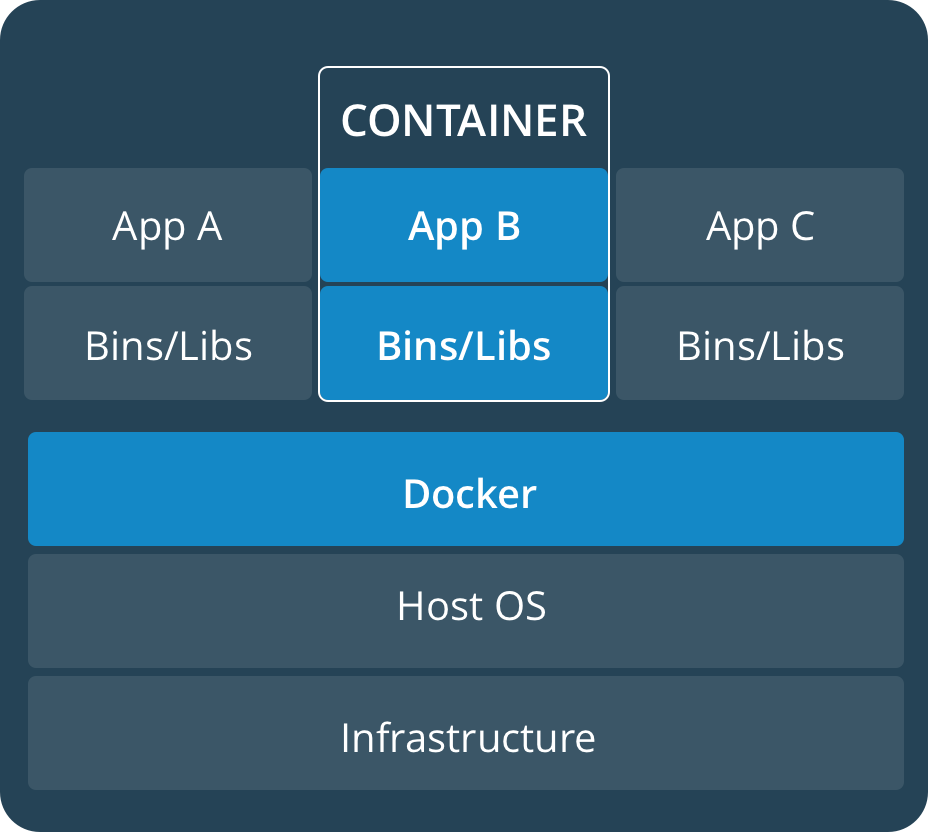
\includegraphics[width=0.70\columnwidth]{img/Container@2x.png}
		\caption{Solution stack di Docker.}
		\label{img:structDoc2}
	\end{center}
\end{figure}
Docker implementa una architettura client–server. Il client è un semplice strumento a linea di comando che invia comandi al server utilizzando servizi REST: questo implica che chiunque potrebbe costruire client differenti. Il server è un daemon Linux in grado di costruire immagini ed eseguire container sulla base di una immagine preesistente.\\Vedi figura: \ref{img:API} \ref{img:registry}
\begin{figure}[H]
	\begin{center}
		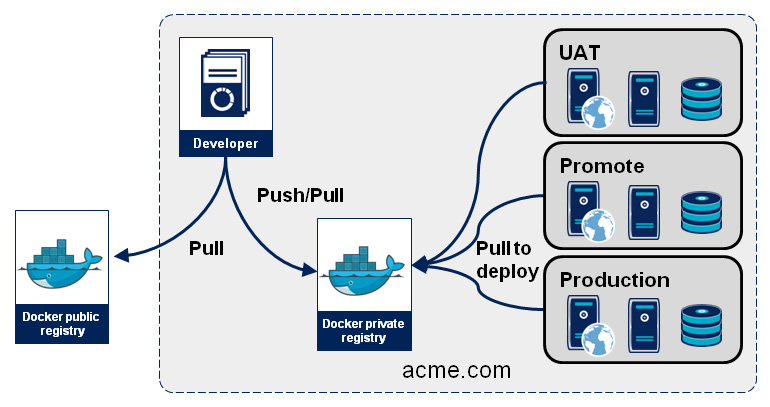
\includegraphics[width=0.99\columnwidth]{img/ContainersOperations-2_fig01.jpg}
		\caption{I registry di Docker.}
		\label{img:registry}
	\end{center}
\end{figure}



\subsubsection{Cenni sulla struttura del FS}
\textbf{Union File System}:
Una caratteristica davvero interessante di Docker è il modo in cui viene gestito il file system. Docker utilizza un’implementazione di \href{https://en.wikipedia.org/wiki/UnionFS}{\textbf{Union File System}} per comporre il file system che apparirà visibile al container. Gli Union File System (ad esempio UnionFS o \href{https://en.wikipedia.org/wiki/Aufs}{\textbf{aufs}}) consentono di unire diversi file system e montarli in un unico punto di mount.\\
Un'immagine Docker è in realtà un insieme di file organizzati in directory: in definitiva, è un file system. Un'immagine docker può essere costruita sulla base di un'immagine già esistente semplicemente aggiungendo e/o modificando alcuni file ad esempio facendo commit di un immagine gia esestende oppure agguingendo strati con il dockerfile. E questo può essere ripetuto per un numero illimitato di volte. Un'immagine può essere ad esempio costituita da $n$ strati (vedi figura: \ref{img:container}): questo concetto è conosciuto anche come “immagini stratificate” \href{http://goo.gl/z1ne3Q}{(\textbf{layered})}. Nell’esempio precedente, quando l’immagine Docker va in esecuzione, i $n$ file system vengono uniti insieme (merge) in modalità sola lettura, e ad essi viene sovrapposto un ulteriore strato in modalità lettura–scrittura writable layer (vedi fig: \ref{img:container}).
\begin{figure}[H]
	\begin{center}
		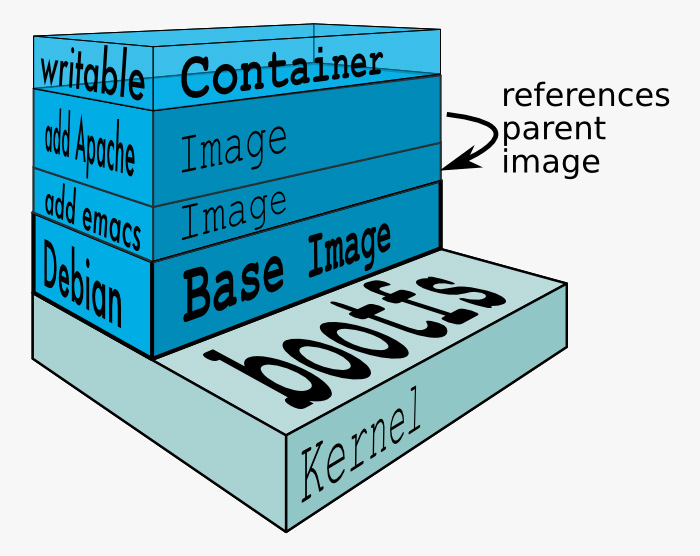
\includegraphics[width=0.99\columnwidth]{img/ContainersOperations-2_fig02.jpg}
		\caption{Un file system stratificato (layered file system).}
		\label{img:layered}
	\end{center}
\end{figure}
Se due container condividono parte degli strati dell’immagine, questi layer non dovranno essere replicati nel file system host, poiché sono montati in modalità sola lettura. Questo può generare significativi risparmi specie se un’azienda si dà una certa disclipina riguardo al modo in cui possono essere create le immagini: potrebbe essere il caso, ad esempio, di stabilire che tutte le immagini debbano derivare da una base comune.\\In questo caso, siccome la base comune sarà probabilmente lo strato che prende la maggior parte dello spazio disco e gli altri layer dovranno aggiungere installazioni o configurazioni minori, tale semplice linea guida potrebbe far risparmiare grandi quantità di spazio disco. Come in figura (\ref{img:layered}) l'immagine di base condivisa fra vari container potrebbe essere quella del layer che comtiene l'immagine Debian. 

\section{Istallare Docker}
Per installare Docker su qualsiasi altra sistema *unix o win seguire la guida ufficiale di Docker \href{https://docs.docker.com/engine/installation/}{https://docs.docker.com/engine/installation/}.
In questo sezione vi mostrerò la procedura per l'installazione dello strumento Docker CE (comiunity edition) su una macchina Ubuntu e come verificare se la procedura sia andata a buon fine. Al fine di non riscontrare problemifuturi è necessario verificare che la versione appena installata sia un varsione maggiore o uguale 1.13.\\Poichè nelle precedenti versioni non sono embedded in docker alcuni tool di automazione e la piattaforma di container scheduling swarmdi cui parleremo più tardi.
\subsubsection {Prerequisiti minimi}Per installare Docker CE è \underline{necessario} avere installato una delle seguenti distribuzioni ubuntu a 64bit in altro casi guarda il link della documentazione ufficiale:
\begin{itemize}
	\item Yakkety 16.10
	\item Xenial 16.04
	\item Trusty 14.04
\end{itemize}
\textbf{1. Step}
\begin{verbatim}

   $ which curl

#  If curl isn’t installed, install it after updating your manager:

   $ sudo apt-get update
   
   $ sudo apt-get install curl

#  Get the latest Docker package.

   $ curl -fsSL https://get.docker.com/ | sh

#  The system prompts you for your sudo password. Then, it downloads and installs Docker and its dependencies.

# Note: If your company is behind a filtering proxy, you may find that the apt-key command fails for the Docker repo
# during installation. To work around this, add the key directly using the following:

   $ curl -fsSL https://get.docker.com/gpg | sudo apt-key add -
     
\end{verbatim}
*IN ADDITION*\\In aggiunta se si vuole si può considerare l'opzione di aggiungere il programma docker alla lista dei programmi con privilegi elevati in modo da poterlo eseguire in modalità non root o senza il comando \texttt{sudo} ogni volta:
\begin{verbatim}

   $	sudo usermod -aG docker <name_of_the_user_to_add>
  	
\end{verbatim}  
Per esempio se si vuole aggiungere l'utente corrente il comando andrà così formattato:
\begin{verbatim}
  
   $  sudo usermod -aG docker `whoami`
    
\end{verbatim}
Ricordati che le modifiche diventeranno effettive solo dopo il logout!\\\\
*PACKAGE EXTRA RACCOMANDATI*\\
L'installazione di questi package extra è necessaria se si vuole montare aufs fisibile anche su docker.
\begin{verbatim}

	$ sudo apt-get update
	
	$ sudo apt-get install curl \
	    linux-image-extra-$(uname -r) \
	    linux-image-extra-virtual

\end{verbatim}
DOPO L'INSTALLAZIONE:\\
procedo con la verifica dell'installazione.\\
procedere con esercizoio di base.\\
Verifica che il servizio docker si in essecuzione sulla tua maccchina ad moogni modo per  sicurezza eseguire la seguente sequenza di comandi:
\begin{verbatim}

	$ sudo service docker status

#next command restart all docker service

	$ sudo service docker restart

\end{verbatim}
In caso arrivati a questo punto per qualche motivo l'istallazine non sia andata a buon fine si potrebbe provare con questa sequenza di comandi:\\
1. Set up del repository\\
Aggiunta di Docker CE repository in Ubuntu. Tramite il seguente comando \texttt{lsb\_release -cs} stampo il nome della mia versione corrente di Ubuntu, esempio "xenial or trusty".
\begin{verbatim}

sudo apt-get -y install \
apt-transport-https \
ca-certificates \
curl

curl -fsSL https://download.docker.com/linux/ubuntu/gpg | sudo apt-key add -

sudo add-apt-repository \
"deb [arch=amd64] https://download.docker.com/linux/ubuntu \
$(lsb_release -cs) \
stable"

sudo apt-get update
\begin{verbatim}
2. Get Docker CE

Install the latest version of Docker CE on Ubuntu:


sudo apt-get -y install docker-ce

\end{verbatim}
*Tratto direttamente dalla documentazione originale (causa recenti aggiornamenti della piattaforma è possibile che alcuni comandi per alcune procedure siano variati nel frattempo invito sempre a verificare sulla documentazione).
\subsubsection{Verifica dell'installazione:}Ora dovremmo essere in grado a lanciare il comando \texttt{doocker run hello-world} e dovremmo ottenere un output tipo questo:
\begin{verbatim}

	$ docker run hello-world
	
	Hello from Docker!
	This message shows that your installation appears to be working correctly.
	
	To generate this message, Docker took the following steps:
	...(snipped)...
	
\end{verbatim}
Iinfine per motivi di compatibilità e per evitare problemi con l'esecuzione di Swarm in docker sucessivamente, accertiamoci di che la versione sia uguale o superiore alla 13.0 eseguendo  il comando \texttt{docker --version} e se vogliamo maggiori informazioni ppossiamo digitare il comando \texttt{docker info}.
\begin{verbatim}

	$ docker --version
	Docker version 17.05.0-ce-rc1, build 2878a85

\end{verbatim}
Arrivati a questo punto si è pronti per iniziare a sperimentare passsando alla sezione dove creeremo di persona le nostre immagini.


\section{Creare un container con Docker}
Inizialmente controlliamo di aver installato docker e che sia la versione giusta come descritto del capitolo precedente.\\
1. Step:\\
Usiamo subito alcuni comandi di base in un semplice esempio alcuni di questi li acciamo già usati:
\begin{verbatim}

1	$ docker run hello-world
2	
3	$ docker --version
	Docker version 17.05.0-ce-rc1, build 2878a85

\end{verbatim}
Ora analizziamo brevente cosa è successo quando abbiamo lanciato sulla nosta macchina per la prima volta un container docker.
Se non ci siamo accorti di averlo fatto è tutto normale, anche perchè non si direbbe che in pochi secondi dal lancio del comando fino allo scaricaricamento dell'immagine dal docker registry alla sua esecuzione sia servito così poco tempo e sia stato così facile.
Il comando che abbiamo lanciato è stato quello alla riga 2(\texttt{docker run hello-world}).
questo comando una volta lanciato a detto a docker di eseguire un containe che conteneva un immagine taggata con il nome di "hello-world", questo a fatto si che il sistema in modo automatico è andato nel repo locale delle immagini e ha cercato se era presente un'immagine con un tag di riferimento "hello-world", ma dato che era la prima volta che la usavamo il sistema non l'ha trovata quindi si è connesso al docker-hub e ha cercato l'immagine da noi richiesta in rete. Una volta trovata l'ha scarica in locale sul nostro host e la eseguita restituendonci a video la banale scritta ciao mondo e qualcos'altro.\\
Esempio di output:
\begin{verbatim}

	test-VirtualBox test \# docker run hello-world
	Unable to find image 'hello-world:latest' locally
	latest: Pulling from library/hello-world
	78445dd45222: Already exists 
	Digest: sha256:c5515758d4c5e1e838e9cd307f6c6a0d620b5e07e6f927b07d05f6d12a1ac8d7
	Status: Downloaded newer image for hello-world:latest
	
	Hello from Docker!
	This message shows that your installation appears to be working correctly.
	
	To generate this message, Docker took the following steps:
	1. The Docker client contacted the Docker daemon.
	2. The Docker daemon pulled the "hello-world" image from the Docker Hub.
	3. The Docker daemon created a new container from that image which runs the
	executable that produces the output you are currently reading.
	4. The Docker daemon streamed that output to the Docker client, which sent it
	to your terminal.
	
	To try something more ambitious, you can run an Ubuntu container with:
	\$ docker run -it ubuntu bash
	
	Share images, automate workflows, and more with a free Docker ID:
	https://cloud.docker.com/
	
	For more examples and ideas, visit:
	https://docs.docker.com/engine/userguide/

\end{verbatim}
Tramite il comando (\texttt{docker images}) possiamo visualizzare le immagini salvate sulla memoria locale del nostro host:
\begin{verbatim}

test-VirtualBox test \#
	docker images
	 
	REPOSITORY          TAG                 IMAGE ID            CREATED             SIZE
	<none>              <none>              8ff43252d7f2        7 weeks ago         191.3 MB
	<none>              <none>              b7a9f1663f67        7 weeks ago         189.3 MB
	<none>              <none>              7ee09435238b        7 weeks ago         188.3 MB
	<none>              <none>              8126e3300de2        7 weeks ago         70.85 MB
	ubuntu              16.04               0ef2e08ed3fa        10 weeks ago        130 MB
	hello-world         latest              48b5124b2768        3 months ago        1.84 kB

\end{verbatim}
Tramite il comando (\texttt{docker rmi <REPO:TAG | IMAGE ID> ...}) possiamo eleiminare le immagini salvate sulla memoria locale del nostro calcolatore.\\\\\\
\begin{verbatim}

test-VirtualBox test \# 
	docker rmi 8ff43252d7f2 b7a9f1663f67 7ee09435238b 8126e3300de2

Deleted: sha256:8ff43252d7f2b4f84785f139e6135df037e731505fd70fc64d00248cbca15bad
Deleted: sha256:b656184f7e21b4dfc6de17aa8df42a0fe01a37df82acd0bbd491dbc529f860b1
	.
	.
	.
Deleted: sha256:7ee09435238ba560fe614d699c33a3532e3ada996ae6c1d9b2d42869525ae3b6
Deleted: sha256:818754db35602595492ef843a644ec16b985b0ab18582b543edc1b4129e0cde8
Deleted: sha256:f91bca33aeae5b04e4235f84459dc933b02268862077ff51d2b2ba4f392be940
==>Error response from daemon: conflict: unable to delete 8126e3300de2 (cannot be forced) - image is being used by running container b3256ad87bc0

test-VirtualBox test \# docker images 
REPOSITORY          TAG                 IMAGE ID            CREATED             SIZE
<none>              <none>              8126e3300de2        7 weeks ago         70.85 MB
ubuntu              16.04               0ef2e08ed3fa        10 weeks ago        130 MB
hello-world         latest              48b5124b2768        3 months ago        1.84 kB

\end{verbatim}
Nel caso la rimozione dell'immagine non vada a buon fine come nel caso (8126e3300de2) basta aggiunger il flag (\texttt{docker rmi --force <REPO:TAG | IMAGE ID> ...})
Ecco una breve riassunto dei principali comandi più usati nella gestione di un container.\\
Una volta installato bisogna far partire il servizio del docker. Su Ubuntu il comando è il seguente:\\
\texttt{service docker start}\\\\
Mentre su altre distro esempio RHEL/CentOS sono questi:\\
\texttt{systemctl enable docker}\\
\texttt{systemctl start docker}\\
Vediamo adesso una serie di comandi (per semplicità solo su Ubuntu, per le altre distribuzioni o sistemi operativi basta consultare la documentazione su https://docs.docker.com/) da utilizzare.\\
\begin{itemize}
\item Per verificare se docker è stato installato correttamente possiamo lanciare il classico "Hello World":
\texttt{docker run hello-world}\\

\item Per stoppare il servizio di docker:\\
\texttt{service docker stop}\\

\item Per cercare un'immagine in Docker Hub:\\
\texttt{docker search <nome\_immagine>}\\

\item Per scaricare un'immagine da Docker Hub:\\
\texttt{docker pull <nome\_immagine>}\\

\item Per scaricare un'immagine da un repository di Docker Hub:\\
\texttt{docker pull <nome\_repository\/nome\_immagine>}\\

 Nei due comandi precedenti si vuole scaricare un'immagine ma non abbiamo indicato il tag, così viene presa l'ultima versione presente dell'immagine. L'uso dei tag viene altamente consigliato perché sono utili soprattutto per l'isolamento e il packaging.\\

\item Il comando con indicazione anche del tag diventa per esempio:\\
\texttt{docker pull <nome\_repository\/nome\_immagine:tag>}\\
\texttt{docker pull ventus85/tomcat:8.0.32}\\

\item Per visualizzare l'elenco delle immagini presenti sulla macchina host:\\
\texttt{docker images}\\

\item Per avviare un nuovo container interattivo che usa la relativa immagine e avvia un terminale all'interno del nuovo container:\\
\texttt{docker run parametri --name <nome\_container> <nome\_immagine:tag>}\\

\item Per esempio se vogliamo avviare il container per tomcat e vogliamo che utilizzi una determinata porta è necessario fare un forwarding. Per fare la mappatura delle porte si usa il parametro "p" mentre per mappare una cartella il parametro è "v".\\
\texttt{docker run -it -d --name tomcat -p 8080:8080 -v \/home\/myApp\/tomcat:\/usr\/local\/tomcat\/log ventus85\/tomcat:8.0.32}\\

\item Quando viene avviato un container esso eseguirà un eventuale entry point (ovvero un file chiamato docker\-entrypoint.sh).
Per avere l'elenco dei container presenti (se aggiungiamo l'opzione -a mostra solo quelli attivi):\\
\texttt{docker ps -a}\\
L'elenco dei contanier contiene:\\
\begin{enumerate}\item l'id del container
\item il nome del container
\item il nome dell'immagine
\item il comando per avviarlo
\item quando è stato creato
\item lo stato (per esempio se è "up")
\item le eventuali porte mappate
\end{enumerate}

\item Se invece vogliamo eseguire un comando su un container che vogliamo eseguire:\\
\texttt{docker exec [OPTIONS] <nome\_container> comando [ARG...]}\\

\item Se per esempio vogliamo aprire una shell per poter usare il container con Oracle:\\
\texttt{docker exec -it oracle bash}\\

\item Per rimuovere un container:\\
\texttt{docker rm <id\_container>}\\

\item Per rimuovere l'immagine:\\
\texttt{docker rmi nome\_immagine}\\

\item Per stampare un file di log del container:\\
\texttt{docker logs <nome\_container>}\\

\item Per avere le informazioni del container (vengono restituite in formato json):\\
\texttt{docker inspect <nome\_container>}\\

\item Per fare un commit (ovviamente in locale) sulle eventuali modifiche effettuate sul container:\\
\texttt{docker commit nome\_container nome\_immagine}\\\\
Questa operazione è utile nel caso si voglia creare una nuova immagine con, per esempio, delle impostazioni diverse rispetto alla precedente.
\end{itemize}
\subsection{Che cos'è il Dockerfile}
Oltre a usare il comando \texttt{commit} per customizzare le nostre immagini e i nostri container è possibile usare il Dockerfile. Esso è un file che crea l'immagine di cui abbiamo bisogno a partire da un'immagine di partenza. Contiene i passaggi da eseguire con il build. La sintassi del docker file è scritta in Ruby più i classici comandi bash.
Riferimento alla guida ufficiale \href{https://docs.docker.com/engine/reference/builder/}{Dockerfile reference}.\\
Una volta creato il nostro Dockerfile (oppure modificato uno precedentemente scaricato), il passo successivo è quello di effettuare il build con un comando come il seguente:
\texttt{docker build -t marco94\/service:fib\_1.0}\\
* Il nome del repository matteo94 l'ho scielto a scopo didattico solo perchè il repo da me creato in quel momento tra i nick-name quello risultava disponibile.
Link del repo su bitbicket \href{https://hub.docker.com/r/matteo94/service/}{https://hub.docker.com/r/matteo94/service/}.

\subsubsection{Come scrivere in semplicità un Dockerfile}
\input{tex/dockerfile.tex}
\chapter{Container orchestration}
Il progetto Docker è nato con l’obiettivo di semplificare la creazione e la gestione di container. Docker svolge questi compiti in modo molto efficace e va riconosciuto al team che l’ha creato la capacità di mantenere l’ambito di questo progetto chiaro e limitato. Docker è un mattone per costruire dei sistemi cloud basati su container.

Costruire un ambiente cloud basato su container implica di tenere presenti alcune aree principali:
\begin{itemize}
\item container scheduling
\item networking avanzato
\item sicurezza
\item monitoraggio
\item quote e misurazioni
\end{itemize}
Vediamo di seguito questi diversi aspetti.
\textbf{Container scheduling}:\\
Il container scheduling (più o meno “calendarizzazione dei container”) è la possibilità di definire e attivare un ambiente potenzialmente composto di diversi container. Come già detto, è un concetto simile a quello dell’orchestrazione negli ambienti cloud basati su Virtual Machine.\\
Attraverso il container scheduling si dovrebbe riuscire a definire la corretta sequenza di attivazione dei container, la dimensione del cluster di container che è necessario creare e la qualità del servizio dei container: per esempio, un’app potrebbe richiedere un minimo garantito di di memoria e di accessi al disco.\\
Tool avanzati per l’orchestrazione devono garantire anche che un determinato ambiente rifletta lo stato desiderato dopo essere stato creato: significa che questi strumenti di orchestrazione possono anche svolgere un certo grado di monitoraggio ed effettuare, almeno in parte, una autoriparazione nel caso lo stato dell’ambiente non si allinei con quello stabilito dalla configurazione.\\
Un’altra importante caratteristica comune a molti scheduler per container è la capacità di definire un livello di astrazione intorno a un cluster di container identici, in maniera tale che essi siano visti come servizio, vale a dire un indirizzo IP e una porta. Questo risultato è ottenuto facendo impostare allo scheduler un load balancer davanti al cluster di container accompagnato dalle regole di indirizzamento necessarie.\\
In quest’ambito, alcuni degli strumenti disponibili sono Swarm e e Docker Compose, Apache Mesos, Kubernetes. Li vediamo di seguito.
\section{Swarm embedded in Docker}
\textbf{Docker Compose}\\
Docker Compose è una aggiunta recente all’insieme delle soluzioni Docker. Compose non può essere considerato ancora pronto per la produzione e non è neanche ben integrato con Docker Swarm, lo strumento di gestione dei cluster targato Docker.\\
Per ora, Docker Compose è in grado di controllare il ciclo di vita di un’applicazione composta di container multipli che sono in esecuzione sullo stesso host.\\
\section{Apache MESOS}
\textbf{Mesos}\\
Mesos è un progetto open source ospitato dalla Apache Foundation. Lo scopo di Mesos sta nel fornire “un sistema kernel distribuito”. Mesos tenta di trasportare i principi del kernel Linux sul sulla temporizzazione dei processi e applicarli a un cluster o a un intero datacenter.\\
Il progetto Mesos è cominciato nel 2012 ed è stato recentemente sottoposto a un processo di reingegnerizzazione per renderlo in grado di gestire i container Docker. Mesos utilizza \href{https://zookeeper.apache.org/}{ZooKeeper} per implementare i concetti dei servizi.\\
Mesos eccelle sulla portabilità ed è possibile creare dei cluster Mesos che si estendono su diversi datacenter e su differenti fornitori di servizi cloud.\\
\section{kubernetes}
\textbf{Kubernetes}\\
Kubernetes è un container scheduler reso disponibile come open source da Google, che afferma di utilizzare i container da circa dieci anni. Kubernetes, in tal senso, rappresenta un modo per condividere con il resto del mondo l’esperienza accumulata in questo periodo.\\
Kubernetes introduce il concetto di pod. I pod sono una serie di container che devono essere collocati insieme nello stesso host. Esistono svariate situazioni o modelli ricorrenti in cui una funzione come questa può essere necessaria: per esempio, un’applicazione potrebbe aver bisogno di un’altra applicazione “di accompagnamento” che si occupi di inviare i log \href{http://blog.kubernetes.io/2015/06/the-distributed-system-toolkit-patterns.html}{pagina del blog in riferimento}.\\
Kubernetes introduce inoltre il concetto di “controller di replicazione”. Il compito di replication controller consiste nel garantire che tutti i pod di un cluster siano “in salute”. Se un pod è giù o non sta fornendo le prestazioni attese, il replication controller lo rimuoverà dal cluster e creerà un nuovo pod.\\
Oltre a questo, Kubernetes cerca di essere portabile tra implementazioni private di Docker e implementazioni cloud pubbliche, grazie all’uso di una architettura a plugin. Per esempio, la configurazione del load balancer necessaria per la definizione di un servizio attiverà un plugin differente a seconda che il deploy del progetto sia effettuato in Google Cloud invece che in Amazon Web Service. L’intenzione è quella di aggiungere plugin per collegarsi a diversi tipi di storage, per effettuare diverse tipologie di deployment, per utilizzare fornitori di sicurezza diversi e così via.\\

%Si può scrivere in \\
%c{grassetto},\\
%\textsc{maiuscoletto}\\
%, in 
%\textit{corsivo},
% \emph{enfatizzato} 
% (ovvero sceglie 
% \LaTeX in base al testo che lo circonda), 
% \underline{sottolineato}, 
% \texttt{equispaziato}
%  (ottimo per il codice, ad esempio 
%  \texttt{public static void main(String[] a)})
%
%\begin{verbatim}
%clear
%clc
%TA=EMGDATA1(1,:);
%GC_filtrato=filtfilt(num,den,GC_abs);
%figure(3);
%plot(TA_filtrato)
%figure(4);
%plot(GC_filtrato)
%for i=1:151
%    EMG_GC_filtrato(1,i)=mean(GC_filtrato(:,(100*(i-1)+1):(100*i)));
%end
%\end{verbatim}
%
%\tiny
%tiny
%
%\scriptsize
%scriptsize
%
%\footnotesize
%footnotesize
%
%\small
%small
%
%\normalsize
%normalsize (default)
%
%\large
%large
%
%\Large
%Large (capital "L")
%
%\LARGE
%LARGE (all caps)
%
%\huge
%huge
%
%\Huge
%Huge (capital "H")
%
%\normalsize
%\begin{equation}
%a_i^n
%\end{equation}


% scegli lo stile, e la bibliografia è gratis
\bibliographystyle{abbrv}
% questo file deve contenere i bibtex.


\bibliography{}

\Large
Documenti di riferimento:\\
\normalsize$- Docker virtualization admin guide.$ (reperoibile in doc/Docker-for-Virtualization-Admin-eBook.pdf)\\
$- Nist definizione di cloud computing.$ (reperibile in/doc/nist-traduzione.pdf)\\

\Large
Siti di riferimento:\\
\normalsize
\label{dockerRegister}\href{http://blog.octo.com/en/docker-registry-first-steps/}{- Primi passi con i registry di Docker}\\
\href{https://it.wikipedia.org/wiki/Docker}{$- https://it.wikipedia.org/wiki/Docker$}\\
\label{nameSpace}\href{http://goo.gl/hLLCoc}{$- http://goo.gl/hLLCoc$}\\
\href{https://it.wikipedia.org/wiki/Comunicazione_tra_processi}{$- https://it.wikipedia.org/wiki/Comunicazione_tra_processi$}\\
\label{LXC}\href{https://it.wikipedia.org/wiki/LXC}{$- https://it.wikipedia.org/wiki/LXC$}\\
\href{https://it.wikipedia.org/wiki/Cloud_computing}{$- https://it.wikipedia.org/wiki/Cloud_computing$}\\
\href{$http://www.cloudtalk.it/container-cosa-sono-come-funzionano$}{$- http://www.cloudtalk.it/container-cosa-sono-come-funzionano$}\\
\href{http://www.cwi.it/data-center/virtualizzazione/container-cosa-funzionano-virtualizzazione-86516}{$- http://www.cwi.it/data-center/virtualizzazione/container-cosa-funzionano-virtualizzazione-86516$}\\

Altri link utili/interessanti:\\
https://it.wikipedia.org/wiki/Docker\\
https://en.wikipedia.org/wiki/Docker\_(software)\\
https://www.zoomingin.net/installiamo-docker-su-ubuntu/\\
http://www.html.it/articoli/docker-i-nostri-servizi-in-un-container-a-prova-di-bomba/\\
http://www.html.it/articoli/vagrant-virtualizzazione-e-provisioning-senza-sforzo/\\
https://www.docker.com/what-docker\\
https://www.docker.com/\\
https://www.miamammausalinux.org/2017/01/giochiamo-con-docker/\\
https://github.com/tianon/docker-brew-ubuntu-core/blob/8ec739cf49ac7fb7517d9ba97b04216dc8d8459b/xenial/Dockerfile\\

\Large
Video tutorial di riferimento:
\normalsize\\
\href{https://www.youtube.com/watch?v=VeiUjkiqo9E#t=60}{$- https://www.youtube.com/watch?v=VeiUjkiqo9E\#t=60$}\\

\end{document}